\section{Validation of the NEMO-Pisces model}
\label{sec:pisces}

The ocean fish biomass is strongly influenced by the physical and geochemical state of the ocean. Therefore, it is important to determine whether the NEMO-Pisces model, which is used to force the Apecosm model, reproduces the expected response to ENSO variability. The aim of the present section is to compare the sea-surface temperature and chlorophyll simulated by the model with observation based datasets.

\subsection{Ocean Nino Index and \sst\ signature}
\label{sec:sst}

As a first step, the Ocean Nino Index (ONI\footnote{\url{https://www.cpc.ncep.noaa.gov/data/indices/oni.ascii.txt}}) has been compared with the simulated one, in order to determine whether the timing of simulated ENSO events is consistent with the observed one. The correlation coefficient between the two monthly time-series over the overlapping period (1958-2018) is $0.94$, which gives confidence in the model ability to reproduce the observed ENSO variability. \\

In order to infer the spatial \sst\ pattern associated with the ONI index, covariance between the ONI index and the NEMO-Pisces \sst\ has been computed. Since the main focus is on the interannual variability, the covariances are applied on yearly time series. The ONI index has been averaged over boreal winter (from November to January), when most of the ENSO variability occurs. In order to insure continuity over the winter months, when ENSO variability usually peaks, yearly means of physical and biogeochemical variables have been computed from May (year $y$) to April (year $y + 1$), as done in \cite{racaultImpactNinoVariability2017}. Then, the obtained time-series has been detrended.\\

The correlation between the ONI index and the sea-surface temperature is shown in figure \ref{fig:cov-sst}. For comparison, the same analysis has been performed with the Hadley SST dataset \citep{raynerGlobalAnalysesSea2003}.
The covariance patterns are very similar between Hadley and simulated SST, with warm anomalies (1\degree C) centerred at the equator and extending from 0 to 90\degree E and from 10\degree S to 10N.\ 
The covariance along the equatorial temperature section (not shown) shows that the maximum temperature anomalies is at around 50m depth at a longitude of 70\degree E. Negative anomalies (-0.8\degree C) are located on the western part of the basin (20\degree W). This dipolar structure is consistent with a shoaling of the thermocline in the west and a deepening in the east.\\

\begin{figure}[h!]
	\centering
	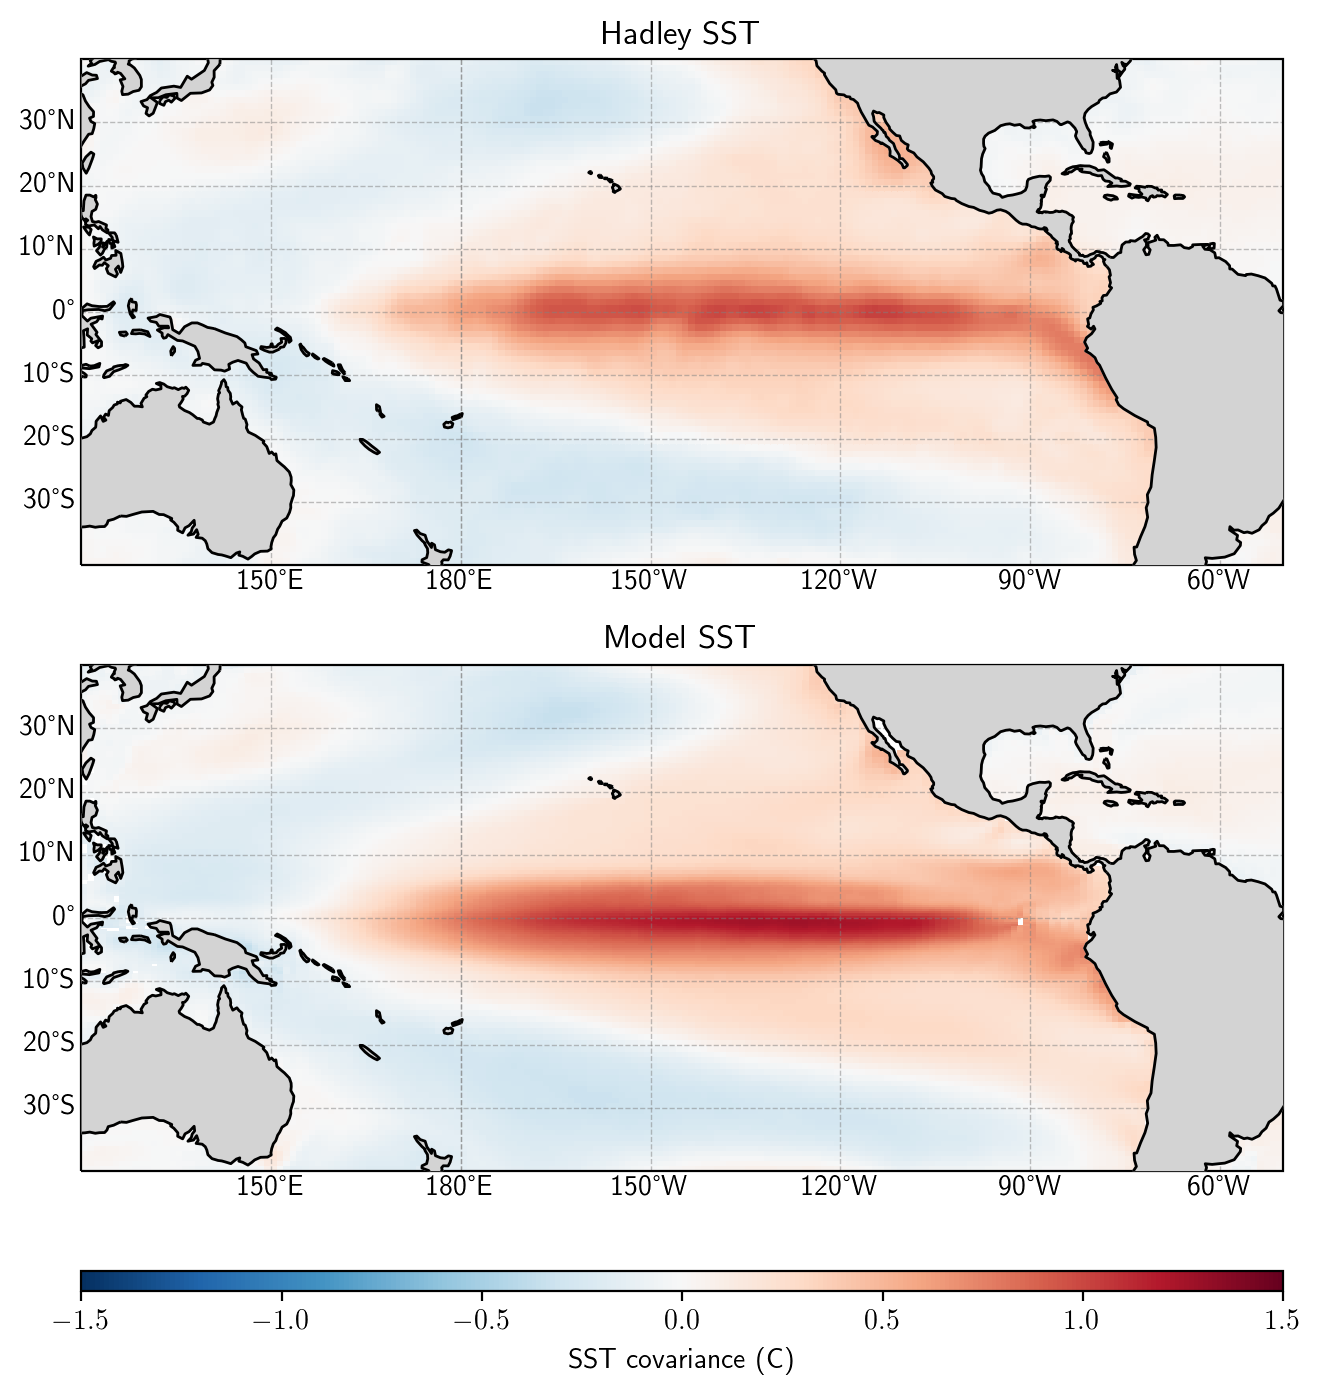
\includegraphics[scale=0.75] {scripts/cov-hadley/covariance_maps_hadley_model.png}
	\caption{Covariance between winter ONI index and Hadley (top) and simulated (bottom) yearly SST anomalies.}
	\label{fig:cov-sst}
\end{figure}

\subsection{Observed and simulated sea-surface chlorophyll}

In order to validate the biogeochemical response of the NEMO-Pisces model, satellite based observations of ocean colour \citep{sathyendranathOceanColourTimeSeries2019} have been used. The OceanColour-CCI V5 dataset provides monthly chlorophyl-a with a horizontal resolution of $1/24$\degree . First, data were Pacific-centerred and regridded to a one degree resolution. This was done by computing the weighted mean over $24 \times 24$ boxes, the weights being provided by the cosine of latitude. Coarse resolution grid cells that contained more than $1/3$ of missing data were considered as missing. Then, a monthly climatology was computed over the 1998-2020 period and removed from the observations. Finally, the covariance between these monthly anomalies and the monthly ONI index was computed between 1997-09 and 2018-12.  In a similar way, the covariance between the ONI index and the simulated surface chlorophyll was computed over the same period.

Covariance maps between the surface chlorophyll and the monthly ONI index are shown in figure \ref{fig:chl-cov}. The observations (upper panel) and the model (lower panel) show very similar covariance pattern, with a decrease in chlorophyll concentration in the tropical Pacific ocean, which is consistent with a reduction of the equatorial upwelling induced by the reduction and eventually reversal of the trade winds (\warn{REF}). However, the model overestimates the chlorophyll response to ENSO variability compared with observational based estimates. Note that the covariance for the simulated chlorophyll has also been computed over the entire simulated period (1958-2018), with no significant changes in the resulting pattern (not shown). \\

\begin{figure}[h!]
	\centering
	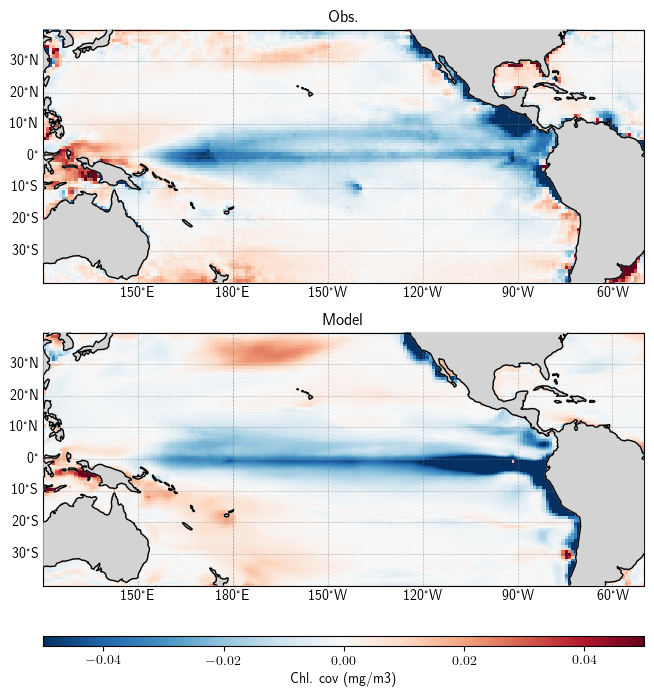
\includegraphics[scale=0.75] {scripts/chl-sat/compare_covariance_chl.png}
	\caption{Covariance between the monthly ONI index and the monthly surface chlorophyll anomalies, computed between 1997-09 and 20018-12.}
	\label{fig:chl-cov}
\end{figure}



%monthly anomalies of simulated sea-surface chlorophyll, averaged between 2\degree S and 2\degree N, has been compared with satellite-based observations \citep{sathyendranathOceanColourTimeSeries2019}. Time-longitude \hov\ diagrams of sea-surface chlorophyll anomalies for both simulated and observed chlorophyll are shown in figure \ref{fig:hov_chl}. Since satellite based observations are provided with a high resolution (1/24\degree), they have been interpolated to a 
%1\degree resolution, in order to be consistent with the model resolution.
%
%\begin{figure}[h!]
%	\centering
%	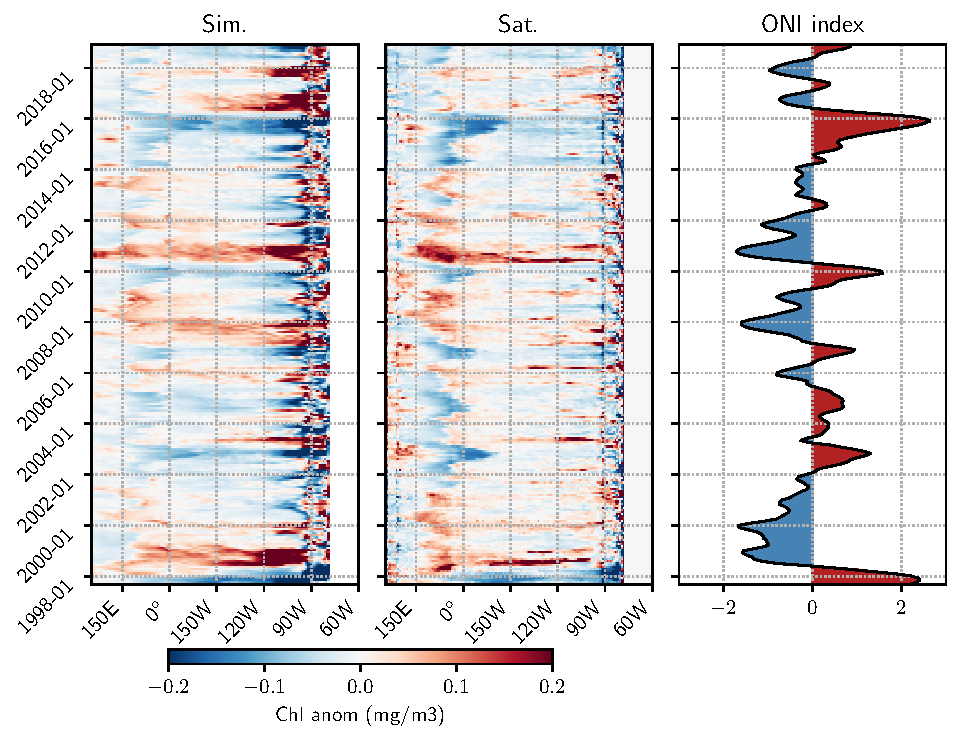
\includegraphics[scale=0.75] {figs/hov_chl.pdf}
%	\caption{}
%	\label{fig:hov_chl}
%\end{figure}
%
%The visual inspection of figure \ref{fig:hov_chl} indicates that at first order, the NEMO-Pisces captures the main patterns of tropical sea-surface chlorophyll variability, although the simulated amplitudes are overestimated. This is further confirmed by a temporal correlation analysis (not shown) between the observed and simulated monthly time series. The correlation coefficients varies between 0.7 and 0.5 between 150\degree E and 100\degree W, and drops below 0.4 west of 150\degree E and east of 100\degree W. \warn{Explain why. Problem with coastal satellite obs?}


%\subsection{Ocean Nino Index and biogeochemical signature}
%
%In order to infer the spatial patterns of the interannual biogeochemical response to ENSO variability, the same covariance analysis as in section \ref{sec:sst} has been performed on yearly (May to April) detrended profiles of biogeochemical variables, averaged between 2\degree S and 2\degree N.\\
%
%Oxygen covariance patterns shows an increase in the oxygen concentration in the eastern part of the basin (90E) between 0 and 200m. This increase of oxygen concentration 
%is consistent with shoaling of the Oxygen Minimum Zone during \nino\ conditions associated with vertical displacements of the thermocline \citep{leungENSODrivesNearsurface2019, espinoza-morriberonOxygenVariabilityENSO2019}. \\
%
%Covariance patterns for phytoplankton variables show that nano-phytoplankton and diatoms (figures \ref{fig:cov-prof}c and \ref{fig:cov-prof}d) respond in different ways to ENSO variability. Small phytoplankton shows negative anomalies between 0 and 80E in near the surface, and positive anomalies at depth (100m). On the other hand, diatoms show negative anomalies which are confined mainly near the surface in the eastern pacific (80E).\\
%
%Zooplankton shows, as nano-phytoplankton, a decrease at the surface, and an 
%increase at lower depth, the latter being more pronounced for micro-zooplankton than for meso-zooplankton (figures \ref{fig:cov-prof}e and \ref{fig:cov-prof}f). The strongest negative anomalies 
%are located near the equator for micro-zooplankton, while they are located at around 90E for meso-zooplankton. 
%Interestingly, the covariance patterns of nano-phytoplankton and micro-zooplankton on the one hand, and of diatoms and meso-zooplankton on the other hand, bear strong resemblance (compare figures \ref{fig:cov-prof}c-\ref{fig:cov-prof}e and \ref{fig:cov-prof}d-\ref{fig:cov-prof}f). \warn{Possibly something related with the size????}\\
%
%\begin{figure}[h!]
%	\centering
%	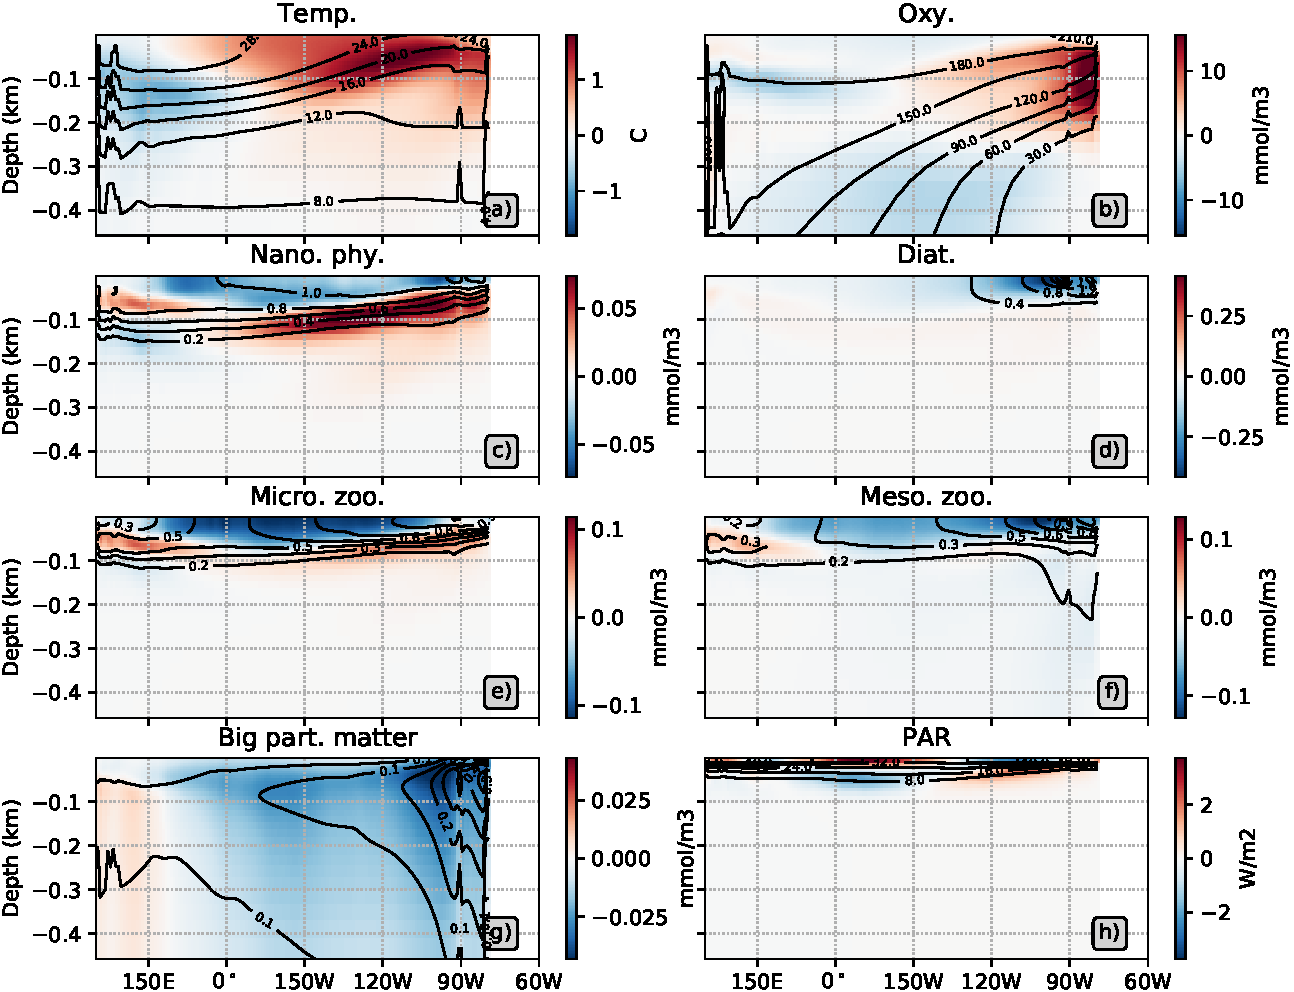
\includegraphics[scale=0.5] {figs/covariance_profiles.pdf}
%	\caption{Covariance between winter ONI index and NEMO-Pisces physical and geochemical variables averaged between 2N and 2S. The mean value is show in black contour lines.}
%	\label{fig:cov-prof}
%\end{figure}
%
%\clearpage
%
%\subsection{Transient response to \nino\ events}
%
%In order to analyse the transient response to \nino\ events, composite analysis has been performed over the most prominent \nino\ years. The latter have been determined as the years durinh which the ONI index averaged from October to December exceeds 1. The obtained years are 1963, 1965, 1972, 1982, 1986, 1987, 1991, 1997, 2002, 2009, and 2015. Because the 1986 \nino\ event extends over two years, 1986 has been removed from the analysis in order to count it only once.\\
% 
%Monthly anomalies (i.e. seasonal cycle removed) have been averaged from January of the \nino\ years ($Y$) to December of the next two years ($Y + 2$). Composite analysis has first been performed on the physical and biogeochemical averaged over the top 200m of the water column and between 2N and 2S. \\
%
%Warm temperature anomalies (figure \ref{fig:hov-pisces}a) seem to originate at around 15E at the onset of \nino and propagate eastward. The maximum warm anomalies are locateds at around 60E and occurr during the december month of the \nino\ event. Cold anomalies are weaker than warm ones and are at their maximum 10 months after the onset of the \nino\ event, at around 40E.
%Contrary to temperature, the oxygen signature of \nino\ events (figure \ref{fig:hov-pisces}b) is limited to the eastern part of the domain, where the \omz\ is situated. At the onset of \nino , oxygen increases sharply (20 $mmol.m^{-3}$). However, around 4 months and 12 months after the \nino\ occurs, the oxygen anomalies are negative and reach -20 $mmol.m^{-3}$. The increase of oxygen can be explained by the shallowing of the highly oxygenated thermocline under \nino\ conditions. \warn{What causes the oxygen decrease? Consumption by plankton? Reduction of PHY, hence no more photo? cf. likeness of O2 and PHY \hov .}.\\
%
%Regarding the response of carbon concentrations, the response of \phy\ and \zoo on the one hand (figures \ref{fig:hov-pisces}c and \ref{fig:hov-pisces}e), and of \phyd and \zood and \goc\ (figures \ref{fig:hov-pisces}d, \ref{fig:hov-pisces}f and \ref{fig:hov-pisces}g) on the other hand, can be regrouped. The formers show positive anomalies in the east during the onset of \nino\ (month 12) in the eastern part of the basin, which are replaced by negative anomalies 4 and 12 months after the beginning of the \nino\ event. One main difference is that in the western part of the domain, \zoo\ shows anomalies which are out of phase with the ones in the east. Furthermore, the eastern anomalies have a smaller zonal extent for \zoo\ than for \phy. The anomalies are of opposed signs for \phyd , \zood\ and \goc\, with negative anomalies in the east during the onset of \nino\, and positive anomalies approximately 4 and 12 months after. \\
%
%Interestingly, the response of \phy\ and \phyd, averaged over the first 200m of the ocean, are in opposite phases. At the onset of \nino, \phy\ increases in the eastern part of the basin (60E - 90E) and shows negative anomalies 4 and 12 months after the beginning of the \nino\ event. The negative anomalies are located westward of the positive ones. The first occurring negative anomalies seem to find their sources between 0 and 30E, before being advected eastward. \\
%
%\warn{Give mechanisms! + references}
% 
%\begin{figure}[h]	
%    \begin{center}
%        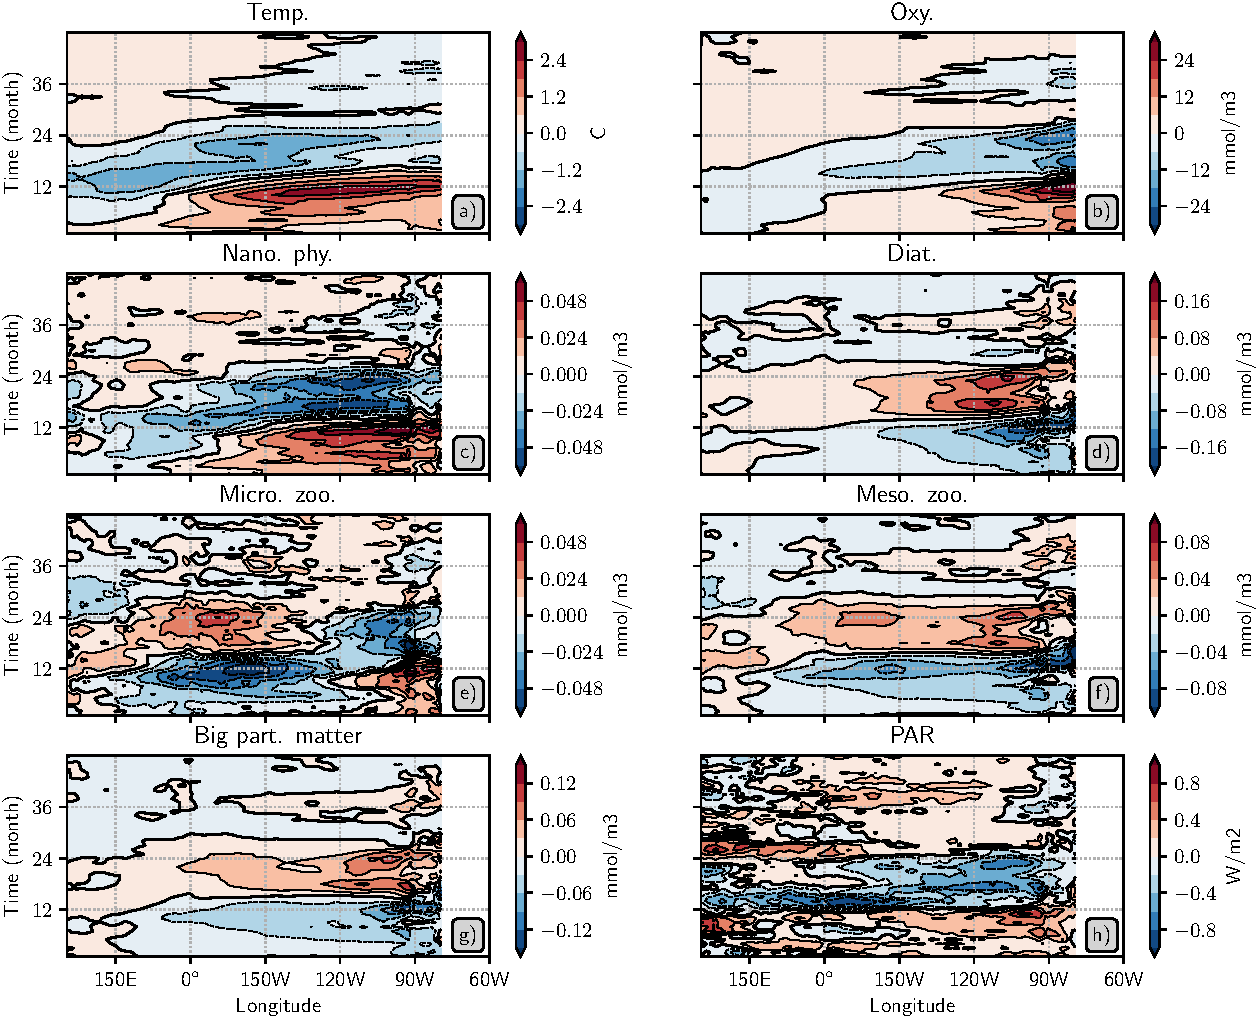
\includegraphics[scale=0.5]{figs/composite_hov_pisces.pdf}
%    \caption{\hov\ diagrams of NEMO-Pisces variables averaged over the top 200m and between 2N and 2S. Month values of 10 to 12 indicate the onset of \nino\ conditions.}
%    \label{fig:hov-pisces}
%    \end{center}
%\end{figure}

\clearpage
